% Yêu cầu 4 — Ngân sách: ~4 trang
\chapter{Kịch bản trình diễn và kết quả}\label{chap:demo}

\section{Phương pháp đánh giá}
Mỗi payload được gửi theo hai đường tới cùng một DVWA (mức bảo mật \textit{low}): trực tiếp qua cổng 8081 (không WAF) và qua WAF ở cổng 8080. Hai đường dùng chung CSDL, chỉ khác nhau ở việc có đi qua ModSecurity hay không, nên mọi khác biệt về kết quả là do WAF. Với mỗi lần gửi, nhóm ghi nhận ba thông tin: mã trạng thái HTTP, việc khai thác có thành công hay không (dựa vào dấu hiệu trong nội dung trả về, ví dụ dòng \texttt{root:x:0:0} của \texttt{/etc/passwd}), và các luật CRS đã khớp trong audit log. Một yêu cầu hợp lệ (\texttt{id=1}) cũng được gửi kèm để kiểm tra WAF không chặn nhầm.

Các bước thực hiện lab như sau:
\begin{enumerate}
\item Khởi động lab: \texttt{cd lab \&\& docker compose up -d}, chờ MariaDB sẵn sàng.
\item Tạo CSDL DVWA qua \texttt{/setup.php} (nút \textit{Create / Reset Database}).
\item Đăng nhập \texttt{admin}/\texttt{password} trên cả hai cổng.
\item Gửi từng payload ở mục~\ref{sec:sqli}--\ref{sec:conlai} theo đường trực tiếp, rồi qua WAF.
\item Đọc audit log bằng \texttt{docker compose logs waf}, lọc theo từng yêu cầu.
\item Đổi \texttt{MODSEC\_RULE\_ENGINE=DetectionOnly}, khởi động lại riêng container \texttt{waf} và lặp lại bước 4--5.
\end{enumerate}
Bước 2--5 được tự động hóa bằng \texttt{lab/scripts/attack.sh}. Script gắn header \texttt{X-Demo-Case} vào mỗi yêu cầu để ghép kết quả với bản ghi audit log tương ứng, rồi lưu toàn bộ bằng chứng (nội dung từng phản hồi, \texttt{audit.json}, \texttt{summary.txt}) vào \texttt{lab/evidence/}.

\section{Kịch bản chi tiết: SQL Injection}\label{sec:sqli}
Trang \textit{SQL Injection} của DVWA ghép tham số \texttt{id} thẳng vào câu truy vấn. Nhóm gửi payload kinh điển \texttt{id=1' OR '1'='1}, làm điều kiện \texttt{WHERE} luôn đúng. Khi gửi trực tiếp, DVWA trả về toàn bộ năm người dùng trong bảng \texttt{users} thay vì một (Hình~\ref{fig:sqli}a). Khi gửi qua WAF, yêu cầu bị chặn với mã 403 trước khi tới DVWA (Hình~\ref{fig:sqli}b).

\begin{figure}[!htb]
\centering
\begin{subfigure}[b]{0.5\linewidth}
\centering
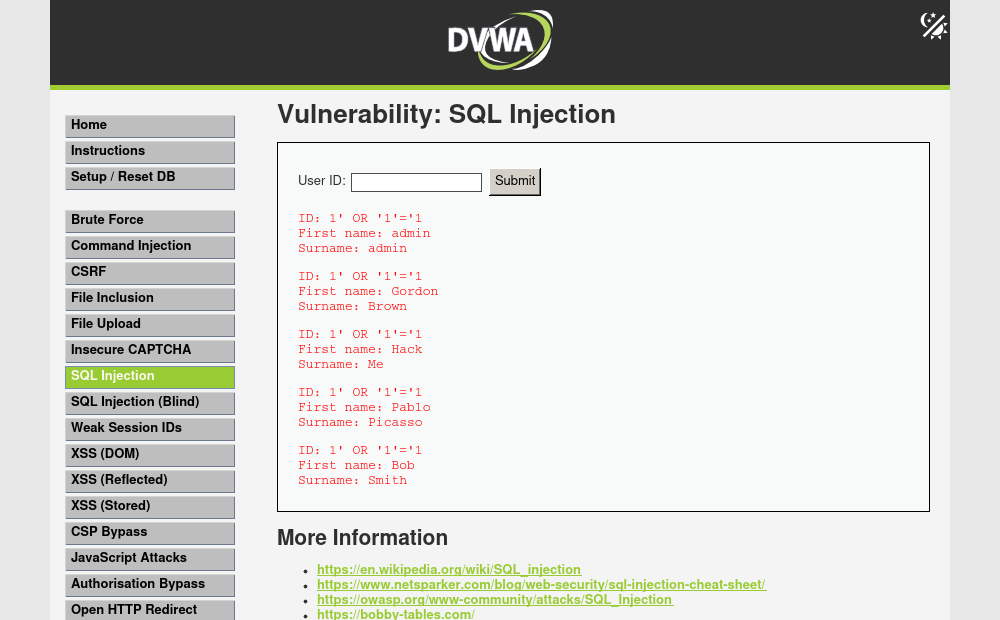
\includegraphics[width=\linewidth,trim=260 150 60 95,clip]{sqli-direct}
\caption{Không WAF: lộ toàn bộ bảng \texttt{users}}
\end{subfigure}\hfill
\begin{subfigure}[b]{0.36\linewidth}
\centering
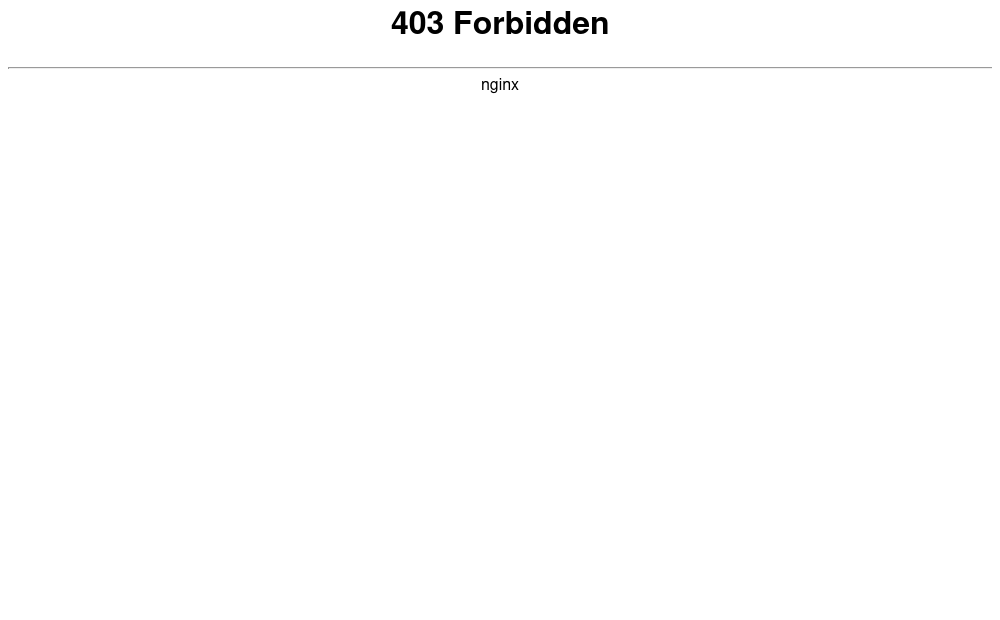
\includegraphics[width=\linewidth,trim=250 500 250 0,clip]{sqli-waf}
\caption{Qua WAF: 403 Forbidden}
\end{subfigure}
\caption{Cùng payload SQLi gửi tới DVWA trực tiếp và qua WAF}
\label{fig:sqli}
\end{figure}

Listing~\ref{lst:audit-sqli} là bản ghi audit log của yêu cầu bị chặn (đã lược bớt các trường không liên quan).

\begin{lstlisting}[caption={Audit log JSON của yêu cầu SQLi bị chặn (rút gọn)},label={lst:audit-sqli}]
{"transaction": {
  "request":  {"uri": "/vulnerabilities/sqli/?id=1%27%20OR%20%271%27%3D%271..."},
  "response": {"http_code": 403},
  "messages": [
    {"message": "SQL Injection Attack Detected via libinjection",
     "details": {"ruleId": "942100", "severity": "2",
       "data": "Matched Data: s&sos found within ARGS:id: 1' OR '1'='1"}},
    {"message": "Inbound Anomaly Score Exceeded (Total Score: 5)",
     "details": {"ruleId": "949110", "severity": "0"}}]}}
\end{lstlisting}

Bản ghi cho thấy đúng cơ chế chấm điểm bất thường đã trình bày ở Chương~\ref{chap:kientruc}. Trong pha 2, luật 942100 gọi libinjection trên tham số \texttt{ARGS:id}; libinjection nhận ra chuỗi token \texttt{s\&sos} (chuỗi -- toán tử -- chuỗi -- toán tử -- chuỗi) đặc trưng cho SQLi. Luật có mức CRITICAL (severity 2) nên cộng 5 điểm. Cuối pha 2, luật 949110 so tổng điểm 5 với ngưỡng \texttt{inbound\_anomaly\_score\_threshold} = 5, thấy đạt ngưỡng nên trả 403. Chỉ một luật khớp cũng đủ chặn, vì ngưỡng mặc định ở PL1 bằng đúng điểm của một luật CRITICAL.

\section{Các kịch bản còn lại}\label{sec:conlai}
\paragraph{Reflected XSS.} Payload \texttt{<script>alert(1)</script>} trong tham số \texttt{name} của trang \textit{XSS (Reflected)}. Không có WAF, DVWA chèn nguyên đoạn script vào trang và trình duyệt thực thi. Qua WAF, bốn luật khớp: 941100 (libinjection phát hiện XSS), 941110 (thẻ \texttt{<script>}), 941160 (chèn HTML) và 941390 (gọi hàm JavaScript \texttt{alert(}), tổng 20 điểm.

\paragraph{Local File Inclusion.} Tham số \texttt{page} của trang \textit{File Inclusion} được \texttt{include} trực tiếp, nên \texttt{?page=../../../../../../etc/passwd} in ra nội dung tệp mật khẩu hệ thống. Qua WAF, các luật 930100/930110 (chuỗi \texttt{../} trên tham số và trên URI thô), 930120 (truy cập tệp hệ điều hành nhạy cảm) và 932160 cùng khớp, tổng 30 điểm.

\paragraph{Command Injection.} Trang \textit{Command Injection} chạy lệnh \texttt{ping} với tham số \texttt{ip}. Payload \texttt{127.0.0.1;cat /etc/passwd} (gửi bằng POST) nối thêm lệnh thứ hai sau dấu \texttt{;}. Qua WAF, luật 930120 và 932160 (phát hiện mã shell Unix) khớp, tổng 10 điểm. Cả hai luật đều bắt chuỗi \texttt{etc/passwd}, không phải dấu \texttt{;} hay lệnh \texttt{cat}. Mục~\ref{sec:pl} cho thấy hệ quả: đổi sang một lệnh ngắn khác thì kết quả thay đổi.

\section{Tổng hợp kết quả}
Bảng~\ref{tab:ketqua} tổng hợp kết quả chạy \texttt{attack.sh} ở chế độ Blocking với cấu hình mặc định (PL1, ngưỡng vào 5, ngưỡng ra 4). Cả bốn loại tấn công đều khai thác được khi không có WAF và đều bị chặn khi đi qua WAF; yêu cầu hợp lệ không bị chặn nhầm. Mọi yêu cầu bị chặn đều kèm luật 949110, không liệt kê lại trong bảng.

\begin{table}[!htb]
\centering
\caption{Kết quả chặn tấn công (Blocking, PL1)}
\label{tab:ketqua}
\footnotesize
\begin{tabularx}{\linewidth}{@{}l>{\raggedright\arraybackslash}p{4.6cm}>{\raggedright\arraybackslash}p{1.9cm}ccX@{}}
\toprule
\textbf{Loại} & \textbf{Payload} & \textbf{Không WAF} & \textbf{Có WAF} & \textbf{Điểm} & \textbf{Luật khớp} \\ \midrule
Hợp lệ & \path{id=1} & 200 & 200 & 0 & -- \\
SQLi & \path{id=1' OR '1'='1} & 200, lộ dữ liệu & 403 & 5 & 942100 \\
XSS & \path{<script>alert(1)</script>} & 200, chạy script & 403 & 20 & 941100, 941110, 941160, 941390 \\
LFI & \path{page=../../../../../../etc/passwd} & 200, đọc tệp & 403 & 30 & 930100, 930110, 930120, 932160 \\
CMDi & \path{ip=127.0.0.1;cat /etc/passwd} & 200, chạy lệnh & 403 & 10 & 930120, 932160 \\
\bottomrule
\end{tabularx}
\end{table}

\section{So sánh DetectionOnly và Blocking}
Khi chuyển \texttt{MODSEC\_RULE\_ENGINE} sang \texttt{DetectionOnly} và chạy lại cùng bộ payload, mọi yêu cầu qua WAF đều trả 200 và khai thác thành công như khi không có WAF. Tuy vậy, audit log vẫn ghi đủ các luật khớp và điểm như ở Bảng~\ref{tab:ketqua}, kể cả luật 949110: ModSecurity vẫn đánh giá yêu cầu nhưng không thực hiện hành động chặn.

Kịch bản LFI còn ghi thêm hai luật đầu ra: 953100 (\textit{PHP Information Leakage}, phát hiện thông báo lỗi PHP trong nội dung phản hồi, mức ERROR, 4 điểm) và 959100 (vượt ngưỡng điểm đầu ra 4). Ở chế độ Blocking không thấy hai luật này vì yêu cầu đã bị chặn ở pha 2, phản hồi không bao giờ được sinh ra. Như vậy pha 4 kiểm tra được cả dữ liệu trả về, và DetectionOnly phù hợp để chạy thử trước khi bật chặn, nhằm thống kê luật nào chặn nhầm lưu lượng thật.

\section{Ảnh hưởng của paranoia level}\label{sec:pl}
Nhóm thử thêm payload \texttt{ip=127.0.0.1;id} trên trang \textit{Command Injection}, tức chạy lệnh \texttt{id} thay cho \texttt{cat /etc/passwd}, ở các mức paranoia khác nhau (biến \texttt{BLOCKING\_PARANOIA}), đồng thời gửi lại yêu cầu hợp lệ \texttt{sqli/?id=1}:
\begin{itemize}
\item PL1 và PL2: payload trả 200, lệnh chạy được (trang hiện \texttt{uid=33(www-data)}), không luật nào khớp; yêu cầu hợp lệ trả 200.
\item PL3: payload bị chặn (403, luật 932350); nhưng yêu cầu hợp lệ \texttt{?id=1} cũng bị chặn bởi chính luật này.
\end{itemize}

Với yêu cầu hợp lệ, audit log ghi \texttt{Matched Data: id found within ARGS\_NAMES:id}: luật so khớp cả \emph{tên} tham số, và tên \texttt{id} trùng với tên một lệnh Unix. Đây là ví dụ cụ thể về sự đánh đổi giữa bỏ sót và chặn nhầm khi tăng paranoia level. Cách khắc phục bằng luật loại trừ được trình bày ở mục~\ref{sec:tinhchinh}.
